\documentclass[12pt]{article}
\usepackage[left=1cm, right=1cm, top=2cm,bottom=1.5cm]{geometry} 

\usepackage[parfill]{parskip}
\usepackage[utf8]{inputenc}
\usepackage[T2A]{fontenc}
\usepackage[russian]{babel}
\usepackage{enumitem}
\usepackage[normalem]{ulem}
\usepackage{amsfonts, amsmath, amsthm, amssymb, mathtools,xcolor,accents}
\usepackage{blkarray}

\usepackage{tabularx}
\usepackage{hhline}

\usepackage{accents}
\usepackage{fancyhdr}
\pagestyle{fancy}
\renewcommand{\headrulewidth}{1.5pt}
\renewcommand{\footrulewidth}{1pt}

\usepackage{graphicx}
\usepackage[figurename=Рис.]{caption}
\usepackage{subcaption}
\usepackage{float}

%%Наименование папки откуда забирать изображения
\graphicspath{ {./images/} }

%%Изменение формата для ввода доказательства
\renewcommand{\proofname}{$\square$  \nopunct}
\renewcommand\qedsymbol{$\blacksquare$}

%%Изменение отступа на таблицах
\addto\captionsrussian{%
	\renewcommand{\proofname}{$\square$ \nopunct}%
}
%% Римские цифры
\newcommand{\RN}[1]{%
	\textup{\uppercase\expandafter{\romannumeral#1}}%
}

%% Для удобства записи
\newcommand{\MR}{\mathbb{R}}
\newcommand{\MC}{\mathbb{C}}
\newcommand{\MQ}{\mathbb{Q}}
\newcommand{\MN}{\mathbb{N}}
\newcommand{\MZ}{\mathbb{Z}}
\newcommand{\MTB}{\mathbb{T}}
\newcommand{\MTI}{\mathbb{I}}
\newcommand{\MI}{\mathrm{I}}
\newcommand{\MCI}{\mathcal{I}}
\newcommand{\MCR}{\mathcal{R}}
\newcommand{\MJ}{\mathrm{J}}
\newcommand{\MH}{\mathrm{H}}
\newcommand{\MT}{\mathrm{T}}
\newcommand{\MU}{\mathcal{U}}
\newcommand{\MV}{\mathcal{V}}
\newcommand{\MA}{\mathcal{A}}
\newcommand{\MB}{\mathcal{B}}
\newcommand{\MF}{\mathcal{F}}
\newcommand{\ME}{\mathcal{E}}
\newcommand{\MW}{\mathcal{W}}
\newcommand{\ML}{\mathcal{L}}
\newcommand{\MM}{\mathcal{M}}
\newcommand{\MP}{\mathcal{P}}
\newcommand{\VN}{\varnothing}
\newcommand{\VE}{\varepsilon}
\newcommand{\dx}{\, dx}
\newcommand{\dy}{\, dy}
\newcommand{\dz}{\, dz}
\newcommand{\dd}{\, d}


\theoremstyle{definition}
\newtheorem{defn}{Опр:}
\newtheorem{rem}{Rm:}
\newtheorem{prop}{Утв.}
\newtheorem{exrc}{Упр.}
\newtheorem{problem}{Задача}
\newtheorem{lemma}{Лемма}
\newtheorem{theorem}{Теорема}
\newtheorem{corollary}{Следствие}

\newenvironment{cusdefn}[1]
{\renewcommand\thedefn{#1}\defn}
{\enddefn}

\DeclareRobustCommand{\divby}{%
	\mathrel{\text{\vbox{\baselineskip.65ex\lineskiplimit0pt\hbox{.}\hbox{.}\hbox{.}}}}%
}
\DeclareRobustCommand{\ndivby}{\mkern-1mu\not\mathrel{\mkern4.5mu\divby}\mkern1mu}


%Короткий минус
\DeclareMathSymbol{\SMN}{\mathbin}{AMSa}{"39}
%Длинная шапка
\newcommand{\overbar}[1]{\mkern 1.5mu\overline{\mkern-1.5mu#1\mkern-1.5mu}\mkern 1.5mu}
%Функция знака
\DeclareMathOperator{\sgn}{sgn}

%Функция ранга
\DeclareMathOperator{\rk}{\text{rk}}
\DeclareMathOperator{\diam}{\text{diam}}


%Обозначение константы
\DeclareMathOperator{\const}{\text{const}}

\DeclareMathOperator{\codim}{\text{codim}}

\DeclareMathOperator*{\dsum}{\displaystyle\sum}
\newcommand{\ddsum}[2]{\displaystyle\sum\limits_{#1}^{#2}}
\newcommand{\ddssum}[2]{\displaystyle\smashoperator{\sum\limits_{#1}^{#2}}}
\newcommand{\ddlsum}[2]{\displaystyle\smashoperator[l]{\sum\limits_{#1}^{#2}}}
\newcommand{\ddrsum}[2]{\displaystyle\smashoperator[r]{\sum\limits_{#1}^{#2}}}

%Интеграл в большом формате
\DeclareMathOperator{\dint}{\displaystyle\int}
\newcommand{\ddint}[2]{\displaystyle\int\limits_{#1}^{#2}}
\newcommand{\ssum}[1]{\displaystyle \sum\limits_{n=1}^{\infty}{#1}_n}

\newcommand{\smallerrel}[1]{\mathrel{\mathpalette\smallerrelaux{#1}}}
\newcommand{\smallerrelaux}[2]{\raisebox{.1ex}{\scalebox{.75}{$#1#2$}}}

\newcommand{\smallin}{\smallerrel{\in}}
\newcommand{\smallnotin}{\smallerrel{\notin}}

\newcommand*{\medcap}{\mathbin{\scalebox{1.25}{\ensuremath{\cap}}}}%
\newcommand*{\medcup}{\mathbin{\scalebox{1.25}{\ensuremath{\cup}}}}%

\makeatletter
\newcommand{\vast}{\bBigg@{3.5}}
\newcommand{\Vast}{\bBigg@{5}}
\makeatother

%Промежуточное значение для sup\inf, поскольку они имеют разную высоту
\newcommand{\newsup}{\mathop{\smash{\mathrm{sup}}}}
\newcommand{\newinf}{\mathop{\mathrm{inf}\vphantom{\mathrm{sup}}}}

%Скалярное произведение
\newcommand{\inner}[2]{\left\langle #1, #2 \right\rangle }
\newcommand{\linsp}[1]{\left\langle #1 \right\rangle }
\newcommand{\linmer}[2]{\left\langle #1 \vert #2\right\rangle }

%Подпись символов снизу
\newcommand{\ubar}[1]{\underaccent{\bar}{#1}}

%%Шапка для букв сверху
\newcommand{\wte}[1]{\widetilde{#1}}
\newcommand{\wht}[1]{\widehat{#1}}
\newcommand{\ovl}[1]{\overline{#1}}


%%Трансформация Фурье
\newcommand{\fourt}[1]{\mathcal{F}\left(#1\right)}
\newcommand{\ifourt}[1]{\mathcal{F}^{-1}\left(#1\right)}

%%Символ вектора
\newcommand{\vecm}[1]{\overrightarrow{#1\,}}

%%Пространстов матриц
\newcommand{\matsq}[1]{\operatorname{Mat}_{#1}}
\newcommand{\mat}[2]{\operatorname{Mat}_{#1, #2}}

%Оператор для действ и мнимых чисел
\DeclareMathOperator{\IM}{\operatorname{Im}}
\DeclareMathOperator{\RE}{\operatorname{Re}}
\DeclareMathOperator{\li}{\operatorname{li}}
\DeclareMathOperator{\GL}{\operatorname{GL}}
\DeclareMathOperator{\SL}{\operatorname{SL}}
\DeclareMathOperator{\Char}{\operatorname{char}}
\DeclareMathOperator\Arg{Arg}
\DeclareMathOperator\ord{ord}

%Оператор для образа
\DeclareMathOperator{\Ima}{Im}

%Делимость чисел
\newcommand{\modn}[3]{#1 \equiv #2 \; (\bmod \; #3)}
\newcommand{\nmodn}[3]{#1 \not\equiv #2 \; (\bmod \; #3)}

%%Взятие в скобки, модули и норму
\newcommand{\parfit}[1]{\left( #1 \right)}
\newcommand{\modfit}[1]{\left| #1 \right|}
\newcommand{\sqparfit}[1]{\left\{ #1 \right\}}
\newcommand{\normfit}[1]{\left\| #1 \right\|}

%%Функция для обозначения равномерной сходимости по множеству
\newcommand{\uconv}[1]{\overset{#1}{\rightrightarrows}}
\newcommand{\uconvm}[2]{\overset{#1}{\underset{#2}{\rightrightarrows}}}

%% Функция для добавления круга сверху множества
\newcommand{\Circ}[1]{\accentset{\circ}{#1}}

%%Функция для обозначения нижнего и верхнего интегралов
\def\upint{\mathchoice%
	{\mkern13mu\overline{\vphantom{\intop}\mkern7mu}\mkern-20mu}%
	{\mkern7mu\overline{\vphantom{\intop}\mkern7mu}\mkern-14mu}%
	{\mkern7mu\overline{\vphantom{\intop}\mkern7mu}\mkern-14mu}%
	{\mkern7mu\overline{\vphantom{\intop}\mkern7mu}\mkern-14mu}%
	\int}
\def\lowint{\mkern3mu\underline{\vphantom{\intop}\mkern7mu}\mkern-10mu\int}

%%След матрицы
\DeclareMathOperator*{\tr}{tr}

\DeclareMathOperator*{\symdif}{\bigtriangleup}

% Верхние\нижние пределы
\DeclareMathOperator*\lowlim{\underline{lim}}
\DeclareMathOperator*\uplim{\overline{lim}}

\makeatletter
\renewcommand*\env@matrix[1][*\c@MaxMatrixCols c]{%
	\hskip -\arraycolsep
	\let\@ifnextchar\new@ifnextchar
	\array{#1}}
\makeatother


%% Переопределение функции хи, чтобы выглядела более приятно
\makeatletter
\@ifdefinable\@latex@chi{\let\@latex@chi\chi}
\renewcommand*\chi{{\@latex@chi\smash[t]{\mathstrut}}} % want only bottom half of \mathstrut
\makeatletter

\setcounter{MaxMatrixCols}{20}

\begin{document}
\lhead{Математический анализ - \RN{4}}
\chead{Шапошников С.В.}
\rhead{Лекция - 15}
\section*{Мера Хаусдорфа}
\subsection*{Размерность Хаусдорфа}
Пусть мы находимся в $\MR^n$ и $E \subset \MR^n$.
\begin{prop}
	Пусть $0 < \alpha < \beta \leq n$ и $H^\alpha(E) < \infty$, тогда $H^\beta(E) = 0$.
\end{prop}
\begin{proof}
	Возьмем $\delta > 0$ и посмотрим как устроена $H_\delta^\beta(E)$. Пусть $E \subset \cup_j F_j, \, \diam{F_j} \leq \delta$, тогда:
	$$
		H_\delta^\beta(E) \leq \ddsum{j}{}(\diam{F_j})^\beta = \ddsum{j}{}(\diam{F_j})^{\alpha}{\cdot}(\diam{F_j})^{\beta - \alpha} \leq\delta^{\beta - \alpha}{\cdot} \ddsum{j}{}(\diam{F_j})^{\alpha} \Rightarrow
	$$
	$$
		\Rightarrow \dfrac{1}{\delta^{\beta - \alpha}}H_\delta^\beta(E) \leq \ddsum{j}{}(\diam{F_j})^{\alpha} \Rightarrow H_\delta^\beta(E) \leq \delta^{\beta - \alpha}H_\delta^\alpha(E)
	$$
	где последнее верно в силу произвольности $F_j$. По построению верно:
	$$
		H_\delta^\alpha(E) \leq H^\alpha(E) \Rightarrow H_\delta^\beta(E) \leq \delta^{\beta - \alpha}{\cdot} H^\alpha(E) = \delta^{\beta - \alpha}{\cdot}c \xrightarrow[\delta \to 0]{} 0 \Rightarrow H^\beta(E) = \lim\limits_{\delta \to 0+} H_\delta^\beta(E)  = 0
	$$
\end{proof}

\begin{defn}
	Пусть $E\subset \MR^n$, тогда число: 
	$$
		\dim_H{E} = \inf\{\alpha \geq 0 \colon H^\alpha(E) = 0\}
	$$
	где в случае, когда таких $\alpha$ нет, то полагаем по определению: 
	$$
		\dim_H{E} = n
	$$ 
	называется \uwave{размерностью Хаусдорфа}.
\end{defn}

\begin{rem}
	Как только мы сталкиваемся с ситуацией, что $0 < H^\beta(E) < \infty$, то мы сразу делаем два вывода:
	\begin{enumerate}[label = \arabic*)]
		\item $H^\alpha(E) = 0, \, \forall \alpha > \beta$, следует сразу из утверждения выше;
		\item $H^\alpha(E) = \infty,  \, \forall \alpha < \beta$, если $H^\alpha(E) \neq \infty$, то $H^\beta(E) = 0 \Rightarrow$ противоречие;
	\end{enumerate}
	Таким образом, если как-то удалось проверить, что $0 < H^\beta(E) < \infty$, то мы сразу знаем, что: $\beta = \dim_H{E}$. Естественно считать, что если удалось $\beta$-мерной мерой Хаусдорфа померить нетривиальное множество, то у него должна быть размерность $\beta$. 
	
	В самом определении размерности не требуется, чтобы при значении равному точной нижней грани, $H^\alpha$ была ненулевой мерой. При всех больших размерностях: $H^\alpha(E) = 0$, а при всех меньших не $0$. Может ли при меньших быть конечное значение?
\end{rem}

\begin{rem}
	Пусть $\beta = \dim_H{E}$, тогда:
	\begin{enumerate}[label = \arabic*)]
		\item 
		$$
			\forall \alpha > \beta, \, H^\alpha(E) = 0
		$$ 
		Это следует сразу из определения и утверждения выше: $\beta$ это точная нижняя грань $\Rightarrow$ сколь угодно близко к $\beta$ встречаются $\wte{\alpha}$, где $H^{\wte{\alpha}}(E) = 0$, а мы знаем, что для всех больших значение меры тоже $0$. Только из определения такой вывод сделать нельзя, поскольку оно говорит лишь про точную нижнюю грань.
		\begin{figure}[H]
			\centering
			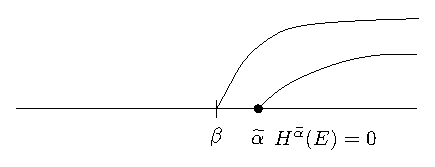
\includegraphics[width=0.35\textwidth]{MA4L15_1.eps}
			\caption{$H^{\alpha}(E) = 0$ при $\alpha > \beta$.}
			\label{15_1}
		\end{figure}
		Берём точку ещё ближе к $\beta$ и так далее, в итоге получаем $0$ на всем промежутке $(\beta,  +\infty)$;
		\item 
		$$
			\forall \alpha < \beta, \, H^\alpha(E) = \infty
		$$ 
		Если $H^\alpha(E) < \infty$, то между $\alpha$ и $\beta$ были бы нули и $\beta$ не было бы точной нижней гранью $\Rightarrow$ противоречие;
		\item Как устроена $H^\beta(E)$ мы не знаем, может быть всё что угодно: может быть конечное число, может быть $0$, может быть $\infty$;
	\end{enumerate}
\end{rem}

\textbf{Пример}: Возьмем $k$-мерную плоскость $\Pi_k \subset \MR^n$, возьмем $H^k$ и множество $E$ на плоскости положительной конечной меры Лебега: $0 < \lambda(E) < \infty$, тогда: $H^k = \lambda_{\Pi_k}$ и верно:
$$
	0 < \lambda(E) < \infty \Leftrightarrow 0 < H^k(E) < \infty \Rightarrow \dim_H E = k
$$
Составим из этих множеств счётную цепочку на этой плоскости так, чтобы: 
$$
	H^k(\cup_n E_n) = \infty
$$ 
При этом будет верно:
$$
	\forall \alpha > k, \, H^\alpha(\cup_n E_n) = 0
$$
Аналогично, можно устроить так, что: 
$$
	\dim_H E = k, \, H^k(E) = 0
$$ 
См. задачу в листке: придумать множество $E \subset \MR$ так, чтобы $\dim_H{E} =1$, но при этом $H^1(E) = 0$. Для этого можно построить множества $E_n$ у которых:
$$
	0 < H^{1 - \tfrac{1}{n}}(E_n) < \infty
$$
И объединение таких $E_n$ и будет искомым множеством $E$: $\cup_n E_n = E$. Основная задача состоит в том, как такие множества построить.

\textbf{Итог}: Когда мы говорим, что какое-то множество имеет размерность Хаусдорфа $k$, то с точки зрения меры Хаусдорфа конкретно про это множество мы ничего сказать не можем, но это говорит нам про меру Хаусдорфа любой большей размерности (что она нулевая) и про меру Хаусдорфа любой меньшей размерности, что она бесконечна. В этом и заключается некоторый способ определить размерность множества через меру Хаусдорфа, но фактически - через покрытия. 

Таким образом, опять используется та же идея, что и в мере Хаусдорфа. Например, как объяснить, что кривая линия это одномерный объект? Это объясняется через покрытие кривой шарами радиуса $\VE$: ищется минимальное возможное покрытие, считается количество шаров и это количество должно себя вести примерно как длина этой кривой, умноженной на $\VE$: $N_\VE \sim 2 L{\cdot}\VE$.

Как можно понять: одномерный это объект или нет? Количество шаров - это величина порядка $\VE$ асимптотически. Если бы объект был бы двумерным, то количество шаров, которые мы использовали бы в покрытии было бы порядка $\VE^2$: $N_\VE \sim c{\cdot}\VE^2$.

\begin{figure}[H]
	\centering
	\includegraphics[width=0.55\textwidth]{MA4L15_2.png}
	\caption{Размерность Хаусдорфа через покрытия.}
	\label{15_2}
\end{figure}
Возникает идея определить непрерывную шкалу размерностей, а именно будем говорить, что у нас размерность $\alpha$, если:
$$
	N_\VE \sim c{\cdot}\VE^\alpha
$$
Это достаточно эвристическое объяснение, строгое приводится с помощью меры Хаусдорфа. Тем не менее, это довольно естественная идея, что когда мы покрываем объект, то количество элементов покрытия связано с размерностью этого множества.

\subsection*{Размерность множества Кантора}

Напомним шаги построения множества Кантора, пусть у нас есть единичный отрезок. На первом шаге отрезок делится на три части, часть посередине удаляется. Получаем два отрезка: $\Delta_{11}$ и $\Delta_{12}$, их объединение:
$$
	Z_1 = \Delta_{11} \cup \Delta_{12}
$$
На следующем шаге, на каждом из оставшихся отрезков повторяется процедура с шага первого: выбрасываются середины и мы получаем уже четыре отрезка: $\Delta_{21}, \, \Delta_{22}, \, \Delta_{23}, \, \Delta_{24}$:
$$
	Z_2 = \Delta_{21}\cup \Delta_{22} \cup \Delta_{23} \cup \Delta_{24}
$$
И так далее, получаем: $Z_n = \cup_k \Delta_{nk}$. Множеством Кантора является пересечение $Z_n$: $C = \cap_n Z_n$. Хотим найти его размерность Хаусдорфа. Попробуем сначала оценить её сверху $H^\alpha(C)$, где $\alpha$ - неизвестно:
$$
	\forall \delta > 0, \, C \subset \bigcup\limits_j F_j, \, \diam{F_j} \leq \delta \Rightarrow H_\delta^\alpha(C) \leq \ddsum{j}{}(\diam{F_j})^\alpha
$$
Возьмем в качестве $F_j$ отрезки $\Delta_{nk}$ для достаточно большого $n$:
$$
	|\Delta_{nk}| = \dfrac{1}{3^n}, \, N_{\Delta_{nk}} = 2^n \Rightarrow \ddsum{j}{}(\diam{F_j})^\alpha = N{\cdot}(|\Delta_{nk}|)^\alpha = 2^n{\cdot}\left(\dfrac{1}{3^n}\right)^\alpha = \left(\dfrac{2}{3^\alpha}\right)^n
$$
Рассмотрим различные случаи для получившегося выражения под скобками:
$$
	\dfrac{2}{3^\alpha} > 1 \Rightarrow \alpha < \log_3{2} \Rightarrow \ddsum{j}{}(\diam{F_j})^\alpha = \left(\dfrac{2}{3^\alpha}\right)^n \xrightarrow[n \to \infty]{} \infty 
$$
Таким образом, самые естественные покрытия приводят к $\infty$. Это не означает, что мы доказали, что мера бесконечная, но наше покрытие в этом смысле плохо работает, возможно надо как-то по-другому покрывать. Тем не менее это сигнал, что такое $\alpha$ лучше не выбирать. Рассмотрим другой вариант:
$$
	\dfrac{2}{3^\alpha} < 1 \Rightarrow \alpha > \log_3{2} \Rightarrow \ddsum{j}{}(\diam{F_j})^\alpha \xrightarrow[n \to \infty]{} 0  \Rightarrow H_\delta^\alpha(C) = 0 \Rightarrow H^\alpha(C) = 0
$$
Получаем: $\dim_H{C} \leq \log_3{2}$. Проверим, что: $\dim_H{C} = \log_3{2}$ и далее считаем, что: $\alpha = \log_3{2}$, тогда:
$$
	\ddsum{j}{}(\diam{F_j})^\alpha = 1 \Rightarrow H^\alpha(C) \leq 1
$$
Таким образом, получили оценку сверху, попробуем получить оценку снизу. Мы знаем, что:
$$
	\forall x \in C, \, x = \ddsum{k = 1}{\infty}\dfrac{2{\cdot}x_k}{3^k}, \, x_k \in \{0,1\}
$$
поскольку Канторовское множество записывается в троичной системе $0$ и $2$. Рассмотрим функцию:
$$
	f\colon C \mapsto [0,1], \, x = \ddsum{k = 1}{\infty}\dfrac{2{\cdot}x_k}{3^k} \mapsto y = \ddsum{k = 1}{\infty}\dfrac{x_k}{2^k} \Rightarrow (0 2 2 2 0 2 \dotsc) \mapsto (0 1 1 1 0 1 \dotsc)
$$
то есть, мы последовательность из $\{0,2\}$ перевели в последовательность из $\{0,1\}$, которую будем трактовать как двоичную запись числа в отрезке $[0,1]$. Отметим, что такое отображение является сюръекцией (но не биекцией!), поскольку получаются всевозможные последовательности нулей и единиц, а следовательно все возможные двоичные записи точек из $[0,1]$. Кроме того, это отображение - непрерывное:
$$
	a,b \in C, \, \dfrac{1}{3^{k+1}} \leq  |a - b| < \dfrac{1}{3^k} \Rightarrow |f(a) - f(b)| \leq \dfrac{1}{2^k}
$$
Это так, посколку правое неравенство для $|a-b|$ означает, что $a$ и $b$ совпадают на первых $k$ цифрах, а значит двоичная запись у $f$ совпадает на первых $k$ цифрах $\Rightarrow$ взять близкие точки из $C$ означает зафиксировать начало троичной записи $\Rightarrow$ зафиксировать начало двоичной записи в образе $\Rightarrow$ отображение непрерывно. Попробуем дать более точную оценку:
$$
	\left(\dfrac{1}{3^{k+1}}\right)^\alpha \leq |a - b|^\alpha, \, \alpha = \log_3{2} \Rightarrow \left(\dfrac{1}{3^{k+1}}\right)^\alpha = \dfrac{1}{2^{k+1}} \Rightarrow \dfrac{1}{2^k} \leq 2{\cdot}|a - b|^\alpha \Rightarrow
$$
$$
	\Rightarrow |f(a) - f(b)| \leq \dfrac{1}{2^k} \leq 2{\cdot}|a - b|^\alpha
$$
Рассмотрим отрезок $[0,1]$, на нем значения функции $f$ принимает значения:
$$
	f\left(\dfrac{1}{3}\right) = f(0222\dotsc) = (0111\dotsc) = \dfrac{1}{2}
$$
$$
	f\left(\dfrac{2}{3}\right) = f(2000\dotsc) = (1000\dotsc) = \dfrac{1}{2}
$$
Аналогично в других точках степени $\tfrac{1}{3}$. При этом: $f(0) = 0, \, f(1) = 1$. Если мы доопределим функцию константой между точек, то мы получим лестницу Кантора.

Обычно лестница Кантора строится через определение интервалов, а дальше доопределяем функцию в остальных точках. Здесь же мы сделали всё наоборот - сначала определили функцию в точках Канторовского множества, а потом уже доопределили на интервалах. То есть, мы взяли лестницу Кантора и ограничили на Канторовском множестве $\Rightarrow$ получили $f$.

\begin{figure}[H]
	\centering
	\includegraphics[width=0.25\textwidth]{MA4L15_3.eps}
	\caption{Лестница Кантора.}
	\label{15_3}
\end{figure}
Геометрически мы склеиваем обратно концы интервалов: $\tfrac{1}{3}$ и $\tfrac{2}{3}$ склеились в $\tfrac{1}{2}$, затем следующие интервалы и так далее. То есть из Канторовского множества склеивается отрезок $[0,1]$:
$$
	f(C) = [0,1] \Rightarrow 1 = H^1([0,1]) = H^1(f(C))
$$
где мера Хаусдорфа от отрезка $[0,1]$ это тоже самое, что и мера Лебега. По аналогии с липшицевыми функциями с прошлой лекции (см. утверждение $3$, лекция $14$):
$$
	C \subset \bigcup\limits_j F_j, \, \diam{F_j} \leq \delta \Rightarrow f(C) \subset \bigcup\limits_j f(F_j) 
$$
$$	
	|f(a) - f(b)| \leq 2{\cdot}|a - b|^\alpha \Rightarrow \diam{f(F_j)} \leq 2{\cdot}\left(\diam{F_j}\right)^\alpha \Rightarrow\ddsum{j}{}\diam{f(F_j)} \leq 2{\cdot}\ddsum{j}{}\left(\diam{F_j}\right)^\alpha \Rightarrow 
$$
$$	
	\Rightarrow H^1_{2\delta^\alpha}(f(C)) \leq 2{\cdot}H_\delta^\alpha(C) \Rightarrow \delta \to 0 \Rightarrow 1 = H^1(f(C)) \leq 2{\cdot}H^\alpha(C) \Rightarrow H^\alpha(C) \geq \dfrac{1}{2} \Rightarrow
$$
$$
	\Rightarrow 0 < H^\alpha(C) < \infty, \, \alpha = \dim_H{C}
$$
\begin{exrc}
	Посчитать размерность Хаусдорфа когда мы каждый раз выбрасываем середину с долей $\gamma$ от всего отрезка, вместо $\tfrac{1}{3}$ как для множества Кантора, где $0 < \gamma < 1$.
\end{exrc}
\begin{exrc}
	Берём множество на отрезке $[0,1]$ такое, что в десятичной записи можно обойтись без $7$. Найти $\dim_H$ этого множества.
\end{exrc}
Что-то по теме можно посмотреть в книгах про фракталы, напримр, посмотреть книгу Кириллова, Фракталы.

\begin{rem}
	Идея с вычислением размерности заключалась в том, что мы выбрали отображение, которое наше сложное множество перевело в множество у которого мы умеем считать меру. И это общий трюк, то есть дальше мы им будем также пользоваться. При этом, чтобы было понятно как связана мера Хаусдорфа до и после отображения нам необходимо, чтобы это отображение каким-то образом позволяло расстояние между образами оценить расстоянием между аргументами, поскольку нужно контроллировать диаметр.
\end{rem}

\newpage
\section*{Интеграл Лебега}

Дальнейший материал будет разбираться менее детальнее, поскольку для него есть отдельный курс действительного анализа.
\begin{defn}
	Пусть у нас есть тройка $(X, \MA,\mu)$, где $\mu$ - $\sigma$-аддитивная, конечная, неотрицательная мера. Эта тройка называется \uwave{измеримым пространством}.
\end{defn}
\begin{defn}
	Функция $f \colon X \to \MR$ называется \uwave{$\MA$-измеримой}, если: $\forall c \in \MR, \, \{x \colon f(x) < c\} \in \MA$.
\end{defn}
\begin{rem}
	Можно показать, что это определение равносильно следующему:
	$$
		\forall B \in \MB(\MR), \, f^{-1}(B) \in \MA
	$$
	Эти моменты обсуждаются на действительном анализе.
\end{rem}

\textbf{Пример}: Если $\MA = 2^X$, то всякая функция измерима.

\textbf{Пример}: Если $\MA = \{\VN, X\}$, то измеримы только константы. Пусть: 
$$
	f(x_1) = y_1 \neq y_2 = f(x_2)
$$ 
тогда будет верно: 
$$
	f^{-1}(\{y_1\}) \neq \VN \wedge f^{-1}(\{y_1\}) \neq X 
$$ 
Следовательно, получили противоречие.

\begin{exrc}
	Пусть $\MA = \{\VN, X, A, X\setminus A\}$, где $\VN \neq A \neq X$. Найти все измеримые функции.
\end{exrc}

На практике обычно берутся очень богатые $\sigma$-алгебры и ситуация практически неотличима от первого примера. Так, например, происходит по мере Лебега: построить неизмеримую функцию достаточно сложно, нужно для начала построить неизмеримое множество (вспомнить про аксиому выбора). 

При этом надо иметь в виду, что измеримость часто используется, например, в теории вероятности, где с помощью неё вводятся ограничения на те или иные отображения, связанные, к примеру, с тем, чтобы утверждать, зависит ли функция от своего поведения на отрезке $[0,t]$ в момент времени $s$ или нет и так далее.

Необходимо иметь в виду, что чтобы сказать, что отображение измеримо, означает во многих случаях ввести серьезное ограничение на это отображение, как во втором примере, где измеримыми функциями могут быть рассматривать только константы.

\begin{theorem}(\textbf{Свойства измеримых функций})
	\begin{enumerate}[label = \arabic*)]
		\item Если $f,g$ - $\MA$-измеримы, тогда: $f + g$ и $f{\cdot}g$ - $\MA$-измеримы;
		\item Пусть $h\colon \MR \to \MR$ - непрерывная функция, а $f$ - $\MA$-измерима, тогда $h(f(x))$ - $\MA$-измерима;
		\item Если $\forall x, \, f(x) = \lim\limits_{n \to \infty}f_n(x)$, $f_n$ - $\MA$-измеримы, то $f$ - $\MA$-измерима;
	\end{enumerate}
\end{theorem}

\begin{exrc}
	Если $h \colon \MR \to \MR$ - непрерывная функция, то $\forall B \in \MB(\MR), \, h^{-1}(B) \in \MB(\MR)$.
\end{exrc}
\begin{proof}
	Рассмтрим все множества $E$, для которых $h^{-1}(E) \in \MB(\MR)$:
	$$
		\MA = \{E \mid h^{-1}(E) \in \MB(\MR)\}
	$$
	Дальше легко проверяется, что $\MA$ это $\sigma$-алгебра, а поскольку $h$ - непрерывная, то эта $\sigma$-алгебра содержит все открытые множества $\Rightarrow$ поскольку борелевская минимальная, то $\MA$ содержит все борелевские множества $\Rightarrow$ проверили, что прообраз борелевского - борелевский.
\end{proof}

\begin{rem}
	Обычно, перед обсуждением измеримости рассматривают две ситуации:
	\begin{enumerate}[label = (\arabic*)]
		\item Имеется множество $X$ с $\sigma$-алгеброй $\MA$ и множество $Y$ без $\sigma$-алгебры. Пусть есть отображение: $f\colon X \to Y$, тогда следующее множество является $\sigma$-алгеброй:
		$$
			 \MB = \{E \subset Y \colon f^{-1}(E) \in \MA\}
		$$
		\item Имеется множество $X$ без $\sigma$-алгебры и множество $Y$ с $\sigma$-алгеброй $\MB$. Пусть есть отображение: $f\colon X \to Y$, тогда следующее множество является $\sigma$-алгеброй:
		$$
			\MA = \{f^{-1}(B) \mid B \in \MB \}
		$$
	\end{enumerate}
	Полезно также доказать, что если имеется отображение $f\colon X \to Y$ и на $Y$ есть некоторое семейство подмножеств $S$, тогда верно:
	$$
		f^{-1}(\sigma(S)) = \sigma(f^{-1}(S))
	$$
	где $\sigma(S)$ - $\sigma$-алгебра порожденная семейством $S$.
\end{rem}

\uline{\textbf{Важный частный случай}}: Пусть $\mu$ - внешняя мера и $\MA_\mu$ - измеримые относительно $\mu$ множества. Тогда измеримые относительно $\MA_\mu$ функции называют $\mu$-\uwave{измеримыми}.

\subsection*{Сходимости измеримых функций}
Пусть $(X,\MA_\mu, \mu)$ - ИП, считаем, что $\mu$ на $X$ - конечна и далее будем рассматривать $\mu$-измеримые функции. Пусть имеется последовательность $f_n$ и функция $f$. У нас будет $3$ вида сходимостей:
\begin{enumerate}[label = (\Roman*)]
	\item \textbf{Равномерная сходимость}: $f_n \uconv{E} f$;
	\item \textbf{Сходимость $\mu$ почти всюду ($\mu$ п.в.)}: $f_n \xrightarrow{\mu \text{ п.в.}} f$, если: $\mu\left(\{x \colon f_n(x) \nrightarrow f\}\right) = 0$;
	\item \textbf{Сходимость по мере}: $f_n \xRightarrow{\mu} f$, если $\forall \delta > 0, \, \mu\left(\{x \colon |f_n(x) - f(x)| \geq \delta\}\right) \xrightarrow[n\to\infty]{} 0$;
\end{enumerate}

\begin{theorem}
	Пусть $\mu$-конечная мера. Тогда:
	\begin{enumerate}[label=\arabic*)]
		\item $(\RN{1}) \Rightarrow (\RN{2}) \Rightarrow (\RN{3})$;
		\item (\textbf{Теорема Егорова}): Если $f_n \xrightarrow{\mu \text{ п.в.}} f$, то:
		$$
			\forall \VE > 0,\, \exists \, X_\VE \colon f_n \uconv{X_\VE} f \wedge \mu(X \setminus X_\VE) < \VE
		$$
		\item (\textbf{Теорема Рисса}): Если $f_n \xRightarrow{\mu} f$, то $\exists \, f_{n_k} \colon f_{n_k} \xrightarrow{\mu \text{ п.в.}} f$;
	\end{enumerate}
\end{theorem}


\end{document}